\onehalfspacing
\section{Đề số 6}
\graphicspath{{./img/}}
\begin{bt} 
	Tính hợp lý các biểu thức sau:
	\begin{enumerate}[a.]
		\item $27 \frac{1}{4} \cdot \frac{5}{8}-13 \frac{1}{4} \cdot \frac{5}{8}$
		\item $2\left|\frac{1}{2}-\frac{3}{4}\right|+\sqrt{\frac{4}{9}}$
		\item $\frac{2^2 \cdot 10+2^3 \cdot 6}{2^2 \cdot 15-2^4}$
	\end{enumerate}
	\loigiai{
		\begin{enumerate}
			\item $27 \frac{1}{4} \cdot \frac{5}{8}-13 \frac{1}{4} \cdot \frac{5}{8}=\frac{5}{8}\left(27 \frac{1}{4}-13 \frac{1}{4}\right)=14 \cdot \frac{5}{8}=\frac{35}{4}$
			\item $2\left|\frac{1}{2}-\frac{3}{4}\right|+\sqrt{\frac{4}{9}}=2\left|\frac{1}{4}\right|+\frac{2}{3}=\frac{1}{2}+\frac{2}{3}=\frac{7}{6}$
			\item $\frac{2^2 \cdot 10+2^3 \cdot 6}{2^2 \cdot 15-2^4}=\frac{2^3 \cdot 5+2^3 \cdot 6}{2^2 \cdot 15-2^4}=\frac{2^3(5+6)}{2^2\left(15-2^2\right)}=\frac{2 \cdot 11}{11}=2$ 
		\end{enumerate}
	} 
\end{bt}

\begin{bt}
	Tìm x biết:
	\begin{enumerate}[a.]
		\item $3(x-2)+\frac{2}{5}=4$
		\item $\left|x+\frac{1}{3}\right|-5=7$
		\item $(2 x-1)^7=(2 x-1)^5$
	\end{enumerate}
	\loigiai{
		\begin{enumerate}
			\item $3(x-2)+\frac{2}{5}=4\\[5px] \Leftrightarrow 3(x-2)=4-\frac{2}{5}\\[5px] \Leftrightarrow 3(x-2)=\frac{18}{5}\\[5px] \Leftrightarrow x-2=\frac{6}{5} \Leftrightarrow x=\frac{16}{5}$
			\item $\left|x+\frac{1}{3}\right|-5=7\\[5px] \Leftrightarrow\left|x+\frac{1}{3}\right|=12\\[5px] \Leftrightarrow\left[\begin{array}{c}x+\frac{1}{3}=12 \\[5px] x+\frac{1}{3}=-12\end{array} \Leftrightarrow\left[\begin{array}{c}x=\frac{35}{3} \\[5px] x=-\frac{37}{3}\end{array}\right.\right.$
			\item $(2 x-1)^7=(2 x-1)^5\\[5px] \Leftrightarrow(2 x-1)^5\left((2 x-1)^2-1\right)=0\\[5px] \Leftrightarrow\left[\begin{array}{l}2 x-1=0 \\[5px] {\left[\begin{array}{l}2 x-1=1 \\[5px] 2 x-1=-1\end{array} \Leftrightarrow\left[\begin{array}{l}x=\frac{1}{2} \\[5px] x=1 \\[5px] x=0\end{array}\right.\right.}\end{array}\right.$
		\end{enumerate}
	} 
\end{bt}

\begin{bt}
	Ba đội cùng chuyển một khối lượng gạch như nhau. Thời gian để đội thứ nhất, đội 
	thứ hai và đội thứ ba làm xong công việc lần lượt là 2 giờ, 3 giờ, 4 giờ. Tính số 
	người tham gia làm việc của mỗi đội, biết rằng số người của đội thứ ba ít hơn số 
	người của đội thứ hai là 5 người.
	\loigiai{
		Gọi số người tham gia làm việc của đội thứ nhất, đội thứ hai, đội thứ ba lân lượt là $\mathrm{x} ; \mathrm{y} ; \mathrm{z}$ (giờ).\\[5px]
ĐK: $x ; y ; z>0$\\[5px]
Cùng một khối lượng công việc, số người tham gia và thời gian làm việc tỷ lệ lệ nghịch.\\[5px]
Theo bài ra ta có: $2 \mathrm{x}=3 \mathrm{y}=4 \mathrm{z}$ và $\mathrm{y}-\mathrm{z}=5$
$$
\begin{aligned}
& \frac{y}{\frac{1}{3}}=\frac{z}{\frac{1}{4}}=\frac{y-z}{\frac{1}{3}-\frac{1}{4}}=\frac{5}{\frac{1}{12}}=60 \\[5px]
& \mathrm{y}=20, \mathrm{z}=15, \mathrm{x}=30 \text { (thoả mãn điều kiện bài toán) }
\end{aligned}
$$
Vậy số người tham gia làm việc của đội thứ nhất, đội thứ hai, đội thứ ba lân lượt là 30 người, 20 người, 15 người.
	} 
\end{bt}

\begin{bt}
	Cho tam giác $\mathrm{ABC}$ vuông tại $\mathrm{A}$ với $\frac{A B}{A C}=\frac{3}{4}$ và $\mathrm{BC}=15 \mathrm{~cm}$. Tia phân giác góc $\mathrm{C}$ cắt $A B$ tại $D$. Kẻ $D E \perp B C(E \in B C)$.
	\begin{enumerate}[a.]
		\item Chứng minh $\mathrm{AC}=\mathrm{CE}$.
		\item Tính độ dài $\mathrm{AB} ; \mathrm{AC}$.
		\item Trên tia $\mathrm{AB}$ lấy điểm $\mathrm{F}$ sao cho $\mathrm{AF}=\mathrm{AC}$. Kẻ tia $\mathrm{Fx} \perp \mathrm{FA}$ cắt tia $\mathrm{DE}$ tại $\mathrm{M}$. Tính $D C M$
	\end{enumerate}
	\loigiai{
		$$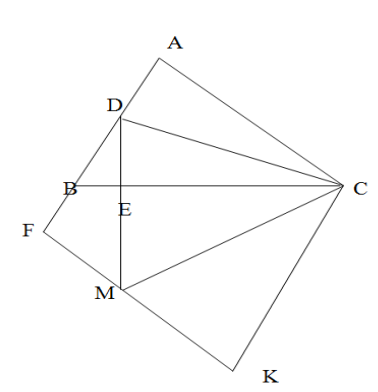
\includegraphics[width=0.45\textwidth]{6-4-lg.png}$$
		\begin{enumerate}
			\item $\mathrm{C} / \mathrm{m}$ được $\triangle A C D=\triangle E C D$ ( cạnh huyền- góc nhọn)\\[5px]
			$\Rightarrow \mathrm{AC}=\mathrm{CE}$ (hai cạnh tưong ứng)
			\item$ \frac{A B}{A C}=\frac{3}{4}(g t) \Leftrightarrow \frac{A B}{3}=\frac{A C}{4} \\[5px]
			 \Leftrightarrow \frac{A B^2}{9}=\frac{A C^2}{16}=\frac{A B^2+A C^2}{9+16}=\frac{B C^2}{25}=\frac{15^2}{25}=9 \\[5px]
			A B^2=9.9=81 \Rightarrow A B=9 \mathrm{~cm} \\[5px]
			A C^2=9.16=144 \Rightarrow A C=12 \mathrm{~cm}
			$
			\item Kẻ $\mathrm{Cy} \perp \mathrm{Fx}$ cắt nhau tại $\mathrm{K}$\\[5px]
			Ta thấy $\mathrm{AC}=\mathrm{AF}=\mathrm{FK}=\mathrm{CK}=\mathrm{CE}$ và $A C K=90^{\circ}$\\[5px]
			C/M được $\triangle C E M=\Delta C K M$ ( cạnh huyên- cạnh góc vuông)\\[5px]
			$\Rightarrow E C M=K C M$ (hai góc tương ứng)\\[5px]
			$
			D C M=D C E+E C M=\frac{1}{2} A C K=\frac{1}{2} \cdot 90^{\circ}=45^{\circ}
			$
		\end{enumerate}
	}
\end{bt}

\begin{bt}
	
	Tìm giá trị lớn nhất của biêu thức: $\mathrm{A}=|x|-|x-2|$
	\loigiai{
		Xét các trường hợp:
		\begin{enumerate}[+]
			\item TH1: $ x \geq 2 \Rightarrow A=x-(x-2)=2$ 
			\item TH2: $ 0 \leq x<2 \Rightarrow A=x+x-2=2 x-2<2$
			\item TH3: $ x<0 \Rightarrow A=-x+x-2=-2<2$
		\end{enumerate}
		$\Rightarrow$ Với mọi giá trị của $\mathrm{x}$ thì $\mathrm{A} \leq 2$\\[5px]
Vậy giá trị lớn nhất của $\mathrm{A}$ bằng 2 khi $\mathrm{x} \geq 2$
	}
\end{bt}